\documentclass[11pt]{article}
\usepackage[margin=1in]{geometry}
\usepackage{amssymb}
\usepackage{amsfonts}
\usepackage{graphicx}

\begin{document}

\title{Definition of Machine Learning}
\author{Kelvin $\cdot$ Liang \, ziyoustep@gmail.com}
\date{June, 6, 2018}
\maketitle

\section{Definition of Machine Learning}
\textbf{Definition: } Design a \emph{Learning Algorithm} that uses \emph{training data} to compute a \emph{hypothesis} $g$ that approximates \emph{target function} $f$

To understand the definition, we need to define some notations.

\begin{enumerate}
\item Input: $x \in X$
\item Output: $y \in Y$
\item Target function: $f: X \to Y$
\item Hypothesis: $g: X \to Y$
\item Hypothesis set: $H$ with $g_0,\cdots, g_k \in H$
\item Training data: $\mathbb{D}=\{(x_1,y_1),\cdots,(x_n,y_n)\}$
\item Learning algorithm: $A$
\end{enumerate}

We are going to explain all these terms in one graph. The graph also shows how they are structured.

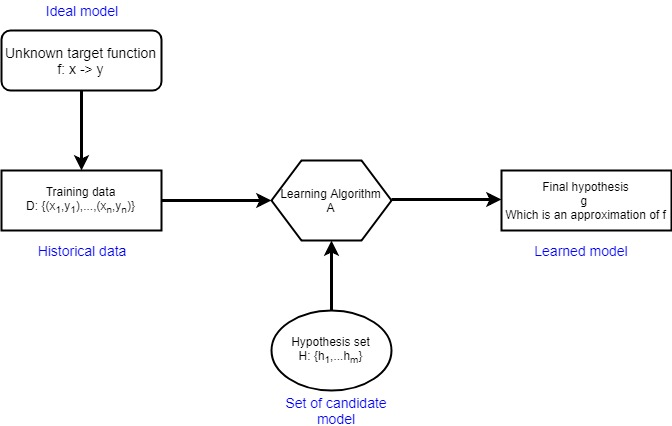
\includegraphics[scale=0.62]{DefinitionOfMachineLearning_graph.jpg}

\section{References}
Almost all of the materials of this note are from Professor Hsuan-Tien Lin , NTU. If you wan to know more information about Machine Learning Foundation, please refer to Professor Lin's homesite.

\end{document}